\documentclass[tikz,border=5mm]{standalone}
\usepackage{amsmath}

\tikzset{
    layer/.style={draw, thick, fill=blue!30},
    process/.style={draw, thick, fill=red!30},
    boundary/.style={draw, thick, fill=black!30}
}

\begin{document}
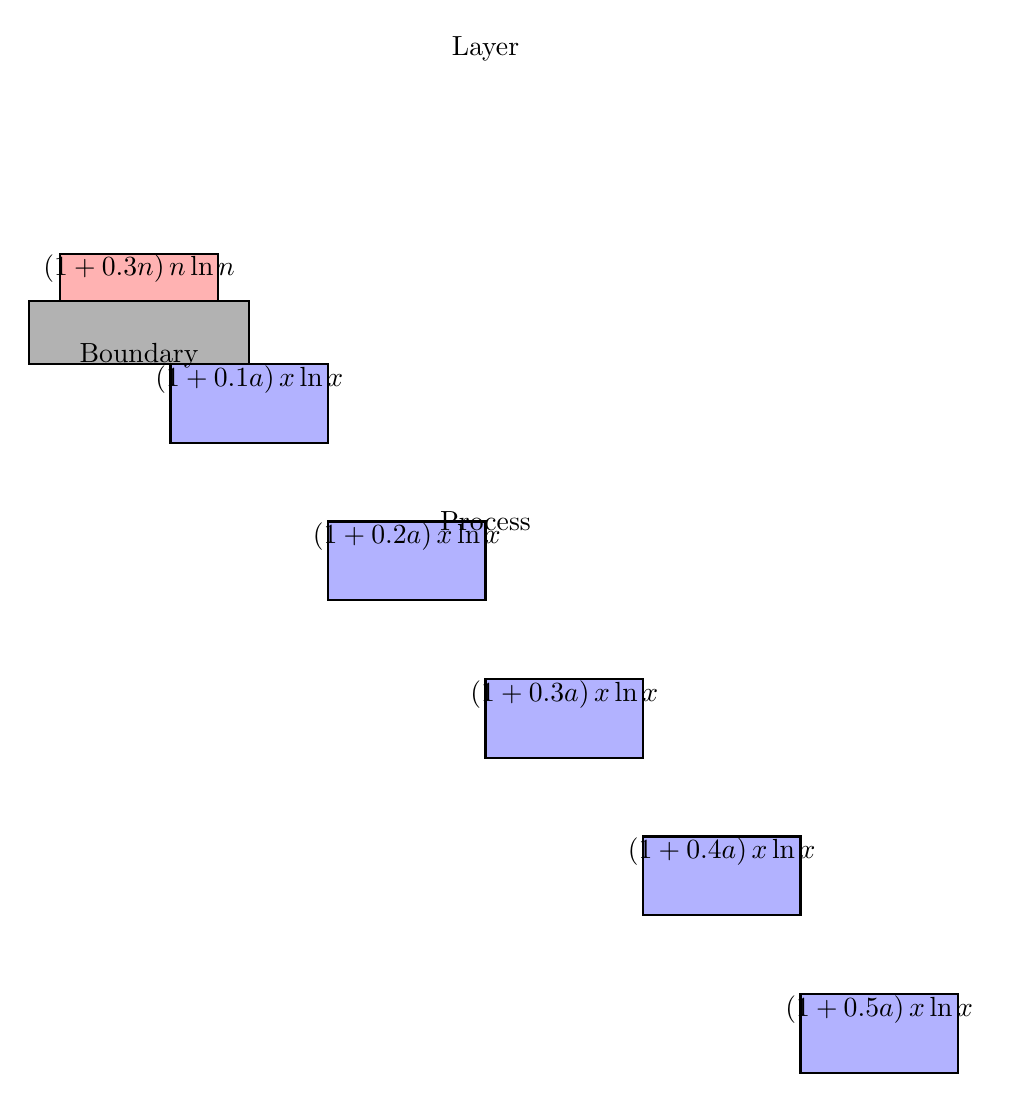
\begin{tikzpicture}[scale=2]

% Draw the layers
\foreach \k [count=\i from 1] in {0.1, 0.2, 0.3, 0.4, 0.5} {
    \draw[layer] (\i-0.5, -\i) rectangle node[midway, above] {$\left(1+\k a\right)x \ln{x}$} (\i+0.5, -\i+0.5);
}

% Highlight the specific layer (1 + a)n ln(n)
\def\a{0.3}
\draw[process] (\a-0.5, -\a) rectangle node[midway, above] {$\left(1 + \a n\right) n \ln{n}$} (\a+0.5, -\a+0.5);

% Block the layer with a black boundary
\draw[boundary] (\a-0.7, -\a-0.2) rectangle node[midway, below] {Boundary} (\a+0.7, -\a+0.2);

% Add labels for clarity
\node at (2.5, 1.5) {Layer};
\node at (2.5, -1.5) {Process};

\end{tikzpicture}
\end{document}